\documentclass{article}

\usepackage[margin=20mm,bottom=20mm,top=20mm]{geometry}
\usepackage{lipsum} % remove me
\usepackage[utf8]{inputenc}
\usepackage{fancyhdr}
\usepackage{lastpage}
\usepackage{multicol}
\usepackage{multirow}
\usepackage{graphicx}
\usepackage[ampersand]{easylist}
\usepackage{float}
\usepackage{tabularx}
\usepackage{textcomp}
\usepackage[table]{xcolor}
\usepackage{hhline}

\pagestyle{fancy}


\definecolor{orange}{HTML}{f2ac45}

\lhead{\includegraphics[width=6cm]{buildbotics_banner.pdf}}
\rhead{CNC Controler Datasheet}

\lfoot{
  \strut\rlap{\color{orange}\rule[-\dp\strutbox]{\headwidth}{0.5cm}}
  www.buildbotics.com
}

\cfoot{\copyright\ Buildbotics LLC, 2016}
\rfoot{Page \thepage\ of \pageref{LastPage}}

\renewcommand{\headrulewidth}{0.4pt}
\renewcommand{\footrulewidth}{0.4pt}

\begin{document}

\begin{multicols}{2}

\hspace*{-1.5cm}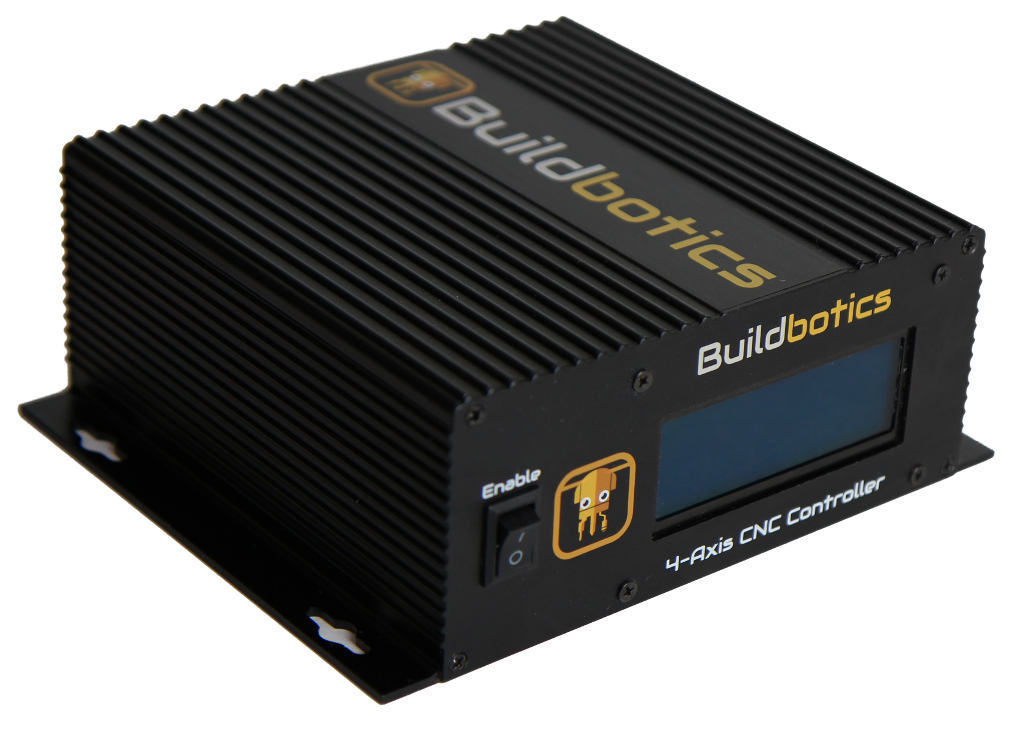
\includegraphics{buildbotics_controller_front_left.png}

\section{Features}
\begin{easylist}[itemize]
& 4-axis stepper motor control
& Up to 800 in/min (20,000 mm/min)
& 12V to 30V supply voltage range
& 4A per channel drive current
& 1/32 microstepping
& Protection features
&& Overcurrent protection
&& Reverse voltage protection
&& Undervoltage lockout
&& Overtemperature motor shutdown
\end{easylist}

\section{Applications}
\begin{easylist}[itemize]
& New CNC designs
& CNC control system upgrades
& 3D printer control
& LASER cutter control
\end{easylist}

\section{Description}
The Buildbotics CNC controller is a feature rich steper motor controller that
is easy to integrate, configure and use.

\lipsum[1-2]

\end{multicols}

\section{Absolute Maximum Ratings}
\begin{table}[H]
\begin{tabularx}{\textwidth}{|X|r r|c|}
\hline
\rowcolor{lightgray}         & MIN     & MAX     & UNIT \\ \hline
Power supply voltage         & -0.6    & 36      & V    \\ \hline
Operating temperature        & -30     & 100     & °C \\ \hline
\end{tabularx}
\label{table:abs}
\end{table}

\section{IO Configuration and Functions}
\begin{table}[H]
\begin{tabularx}{\textwidth}{|l|c|c|X|}
\hline
\rowcolor{lightgray}
\multicolumn{2}{|c|}{\textbf{PIN}} & &
\\ \hhline{|-|-|>{\arrayrulecolor{lightgray}}-|-|>{\arrayrulecolor{black}}}

\rowcolor{lightgray}
\textbf{NAME} & \textbf{NO.} & \multirow{-2}{*}{\textbf{I/O}} &
\multicolumn{1}{c|}{\multirow{-2}{*}{\textbf{DESCRIPTION}}} \\ \hline

\hline
\multicolumn{4}{|l|}{} \\
\multicolumn{4}{|l|}{\textbf{POWER CONNECTOR}} \\ \hline
GND & 1,2 & - & Device ground \\ \hline
Vss & 3,4 & - & Device supply voltage \\ \hline

\hline
\multicolumn{4}{|l|}{} \\
\multicolumn{4}{|l|}{\textbf{MOTOR CONNECTOR}} \\ \hline
A+ & 1 & O & Stepper motor phase A \\ \hline
A- & 2 & O & Stepper motor phase A \\ \hline
B+ & 3 & O & Stepper motor phase B \\ \hline
B- & 4 & O & Stepper motor phase B \\ \hline

\hline
\multicolumn{4}{|l|}{} \\
\multicolumn{4}{|l|}{\textbf{LOAD SWITCH CONNECTOR}} \\ \hline
 & 1 & O &  \\ \hline
 & 2 & O &  \\ \hline
 & 3 & O &  \\ \hline
 & 4 & O &  \\ \hline
 & 5 & O &  \\ \hline
 & 6 & O &  \\ \hline

\hline
\multicolumn{4}{|l|}{} \\
\multicolumn{4}{|l|}{\textbf{IO CONNECTOR}} \\ \hline
 & 1 & O &  \\ \hline
 & 2 & O &  \\ \hline
 & 3 & O &  \\ \hline
 & 4 & O &  \\ \hline
 & 5 & O &  \\ \hline
 & 6 & O &  \\ \hline
 & 7 & O &  \\ \hline
 & 8 & O &  \\ \hline
 & 9 & O &  \\ \hline
 & 10 & O &  \\ \hline
 & 11 & O &  \\ \hline
 & 12 & O &  \\ \hline
 & 13 & O &  \\ \hline
 & 14 & O &  \\ \hline
 & 15 & O &  \\ \hline
 & 16 & O &  \\ \hline
 & 17 & O &  \\ \hline
 & 18 & O &  \\ \hline
 & 19 & O &  \\ \hline
 & 20 & O &  \\ \hline
 & 21 & O &  \\ \hline
 & 22 & O &  \\ \hline
 & 23 & O &  \\ \hline
 & 24 & O &  \\ \hline
 & 25 & O &  \\ \hline
 & 26 & O &  \\ \hline

\end{tabularx}
\label{table:io}
\end{table}

\section{Recommended operating conditions}
\begin{table}[H]
\begin{tabularx}{\textwidth}{|X|r r|c|}
\hline
\rowcolor{lightgray}         & MIN     & MAX     & UNIT \\ \hline
Power supply voltage         & 12      & 30      & V    \\ \hline
\end{tabularx}
\label{table:abs}
\end{table}

\section{Detailed Description}
\lipsum[1-2]

\section{Feature Description}
\lipsum[1-2]


\end{document}
